% Course report in the user's supplied ICRA 2027 ieeeconf template.
\documentclass[letterpaper,10pt,conference]{ieeeconf}
\IEEEoverridecommandlockouts
\overrideIEEEmargins
\usepackage[T1]{fontenc}
\usepackage{mathptmx}
\usepackage{amsmath,amssymb,graphicx,booktabs,cite,url}
\usepackage[hidelinks]{hyperref}
\hypersetup{pdftitle={Text-Driven Humanoid Grasping: Motion Generators and Structured Predictive Residual Control},pdfauthor={DASC7606C Group 3}}
\newcommand{\Risk}{\mathcal{G}_{\phi}}
\newcommand{\Res}{\mathcal{R}_{\theta}}
\newcommand{\ours}{Risk-guided residual}
\title{\LARGE \bfseries Text-Driven Humanoid Grasping:\\Motion Generators and Structured Predictive Residual Control}
\author{DASC7606C Group 3}
\begin{document}
\maketitle
\thispagestyle{empty}
\pagestyle{empty}

\begin{abstract}
We develop a text-driven tabletop grasping system for the Unitree G1, connecting two pretrained motion generators, ARDY and Kimodo, to a common SONIC whole-body controller. On the shared 100-scene benchmark, both generators initially meet the grasp threshold in 58 trials, but Kimodo retains 55 grasps and ARDY 40; ARDY responds faster. We introduce a learned predictive interface between nominal motion and corrective control. A temporal Transformer organizes measured history and upcoming nominal motion into body-by-time risk tokens; a second consumes these predicted tokens to generate bounded arm corrections. In an independent paired evaluation of the ARDY-based system, the learned controller raises end-to-end success from 54/124 (43.55\%) to 74/124 (59.68\%): a 16.13 percentage-point gain, with 25 rescues and five harms. The exact paired result, $p=0.000325$, passes the prespecified threshold of 0.00625. Annotated videos link instructions, execution stages, and both successful and failed object interactions.
\end{abstract}

\section{Introduction}
Natural-language humanoid manipulation combines motion generation with physical execution. A generator can describe how a robot should reach, lower its hand, and lift an object; successful grasping additionally requires accurate finger--object alignment, stable contact, sufficient clearance, and retention throughout the motion. A visually plausible reach can therefore track well and still fail to pick up a block.

We implement this complete route in simulation using ARDY~\cite{ardy} and Kimodo~\cite{kimodo} as two distinct text-to-motion baselines, both executed through pretrained SONIC~\cite{sonic}. A common G1 reference interface, tabletop scene, staged language coordinator, and separate finger controller support the comparison. ARDY provides interactive autoregressive generation conditioned on measured motion history; Kimodo provides controllable kinematic motion diffusion with native spatial constraints. Their different conditioning interfaces expose a practical question: which generated motions remain useful after whole-body tracking and physical hand--object interaction?

Our team visited Archon and learned about S0/S1 models and the simulation-to-robot gap. This experience motivated an execution-side extension that preserves the pretrained motion pipeline. Its central component is a learned predictive interface: Risk combines recent execution and upcoming nominal motion into tokens indexed by future time and body region, and Residual consumes these predicted tokens to request bounded arm corrections. Auxiliary execution prediction trains the representation; correction supervision connects it to physical behavior. A separate scalar head schedules Residual invocation, allowing the same conditioning pathway to operate continuously or selectively.

The design asks whether predicted execution risk can inform both when and how to correct a nominal motion. Our contributions are a shared ARDY/Kimodo-to-SONIC grasping system, a structured predictive interface coupling future-execution prediction to residual correction, and task-level evaluation of both. The baseline comparison uses 100 trials per generator. A separate independent paired confirmation demonstrates a 16.13 percentage-point improvement over ARDY without retraining ARDY or SONIC. A same-weight study compares invocation schedules while preserving structured Risk conditioning. Videos show the text, motion, and object interaction behind these results.

\begin{figure*}[t]
\centering
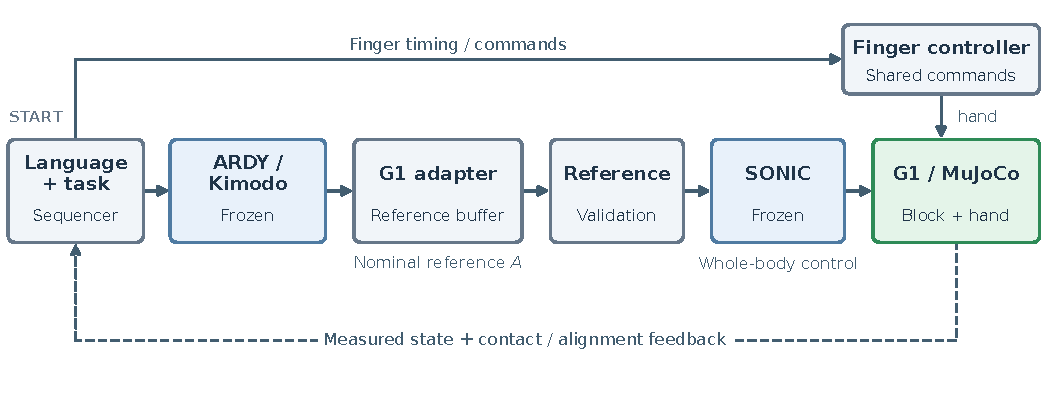
\includegraphics[width=\textwidth]{figures/system.pdf}
\caption{Shared text-to-motion system, read from left to right. ARDY and Kimodo export a common G1 reference interface for frozen SONIC. Stage-specific finger commands follow a separate shared path; measured state and contact feedback support task coordination.}
\label{fig:system}
\end{figure*}

\section{Background and Archon Session}
\subsection{Archon Session}
All team members attended the supervised Archon visit and learned about S0/S1 models, demonstration recording, and policy inference. Archon's whole-body intelligence perspective treats a humanoid as a coordinated embodied system: arm motion depends on posture, balance, contact, and the environment, so a plausible hand trajectory alone does not specify an executable manipulation~\cite{archon_wbi}.

Archon's published hierarchy separates semantic reasoning (S2), native multimodal humanoid modeling (S1), motion generation with a Behavior Foundation Model (S0.5), and motion execution (S0)~\cite{archon_wbi}. This distinction helped us identify two interfaces in our project. ARDY and Kimodo supply movement intent, while SONIC turns adapted references into whole-body control. Our execution-side extension then feeds measured behavior back into the reference through predictive Risk and bounded Residual correction. Its body/time structure connects an upcoming manipulation problem to the region and interval where corrective control can act.

Demonstration recording associates instructions and observations with demonstrated robot states, actions, timestamps, and episode boundaries. During inference, current instructions and observations condition action intent or chunks, which pass through representation conversion and whole-body/hand controllers. The visit made synchronization a central design consideration: learning needs the relationship between what was requested, what was observed, and what the robot actually executed.

The resulting insight is that better generation and better execution address complementary problems. Our simulator exposes object pose and contacts directly; hardware requires sensing and state estimation, calibration, communication timing, and robust contact control. This motivated causal measured-history inputs, future nominal previews, synchronized rollout records, and explicit correction bounds, while keeping motion generation and SONIC frozen.

\subsection{Related Work}
Text-to-motion generation and whole-body control address different interfaces. ARDY's autoregressive diffusion supports interactive conditioning on recent motion, while Kimodo emphasizes controllable generation through spatial and kinematic constraints~\cite{ardy,kimodo}. Their outputs describe desired movement; adapting root orientation, joint order, sampling rate, and contact-sensitive hand goals determines how those outputs enter a robot controller. We compare these deployed systems under one SONIC executor, which supplies pretrained whole-body tracking~\cite{sonic}.

Residual policy learning combines a base controller with a learned corrective action~\cite{residual_policy,residual}. Silver et al. and Johannink et al. study residuals through reinforcement learning; our controller uses supervised targets from verified recovery branches, causal teacher behavior, and stable identity examples. Temporal Transformers~\cite{transformer} encode recent execution together with future nominal motion. Auxiliary execution prediction gives the intermediate representation body and time structure, and the correction model consumes the predicted representation used at runtime.

This separates three design questions: which generator supplies useful nominal motion, whether learned feedback improves its execution, and when that feedback should run. Our generator benchmark, paired controller confirmation, and same-weight invocation ablation provide evidence for these respective questions.

\section{Simulation System and Motion Baselines}


\subsection{Shared Task and Execution Interface}
The MuJoCo~\cite{mujoco} scene uses the Unitree G1 description~\cite{unitree_g1} with a table and a dynamic, unattached block. The nominal setup uses a 6\,cm cube and a 0.70\,m table. A stage coordinator translates the task into reach, lower/alignment, finger closing, lift, and hold instructions. One recorded reach prompt is \emph{``A person stands upright and slowly bends the right elbow, raising the open right hand upward beside the body, then extending the hand forward above the table. Both feet stay planted and the left arm stays at the side.''} Phase prompts and simulator-grounded goals constrain the generated motion. This provides a reproducible staged language task with automated alignment replans.

Both generators export root translation, root quaternion, and 29 named body-joint angles, forming a 36-dimensional configuration. The adapters map joints by name, resample references to 50\,Hz, and recompute velocities after interpolation and transitions. We use the released SONIC execution interface~\cite{sonic_software} for closed-loop whole-body tracking. Learned offsets change only the arms; root, torso, and leg references remain under SONIC, with planted-foot instructions and simulated ground contact supporting stance. Finger articulation is commanded separately using PD control and a 2.5\,rad/s command-rate limit. The block remains governed by simulated contacts rather than an attachment to the hand.

The execution/state clock is 50\,Hz and the physical task evaluator runs at 200\,Hz. SONIC receives ten reference slots spaced by 0.1\,s. Generation pauses simulated time, so command-response wall time and physical control time are measured separately. Generated references are checked against the compiled G1 joint ranges before installation.

\subsection{ARDY and Kimodo Adapters}
\textbf{ARDY.} The frozen ARDY-G1-RP-25FPS-Horizon8 model uses a shared 4,096-dimensional LLM2Vec text embedding~\cite{llm2vec}, measured pose history, and end-effector/posture constraints. Its native motion rate is 25\,Hz and the deployed sampler uses ten denoising steps. Feedback-driven lower replans start from the robot's measured configuration. Native history conditioning makes ARDY a convenient base for the learning extension.

\textbf{Kimodo.} The frozen Kimodo-G1-RP-v1 model generates at 30\,Hz with 100 denoising steps and text/constraint guidance weights of two. Its adapter converts phase goals into native wrist-position, wrist-rotation, and torso-rotation constraints. Measured history anchors the initial heading, state, and transition boundaries; it is not supplied as ARDY-style sequence conditioning. The maximum generated clip has 300 frames. The recorded baseline uses raw generated rotations with its calibrated wrist offset and no static forward-kinematic projection.

These are distinct motion generators sharing SONIC, the scene family, articulated hands, task criteria, and instruction coordinator. Method-specific grounding translates a common task goal into each generator's supported constraints. Both baselines run without additional human corrections; automatic alignment replans remain part of the implementation.

\section{Structured Predictive Risk and Residual Control}
\begin{figure*}[t]
\centering
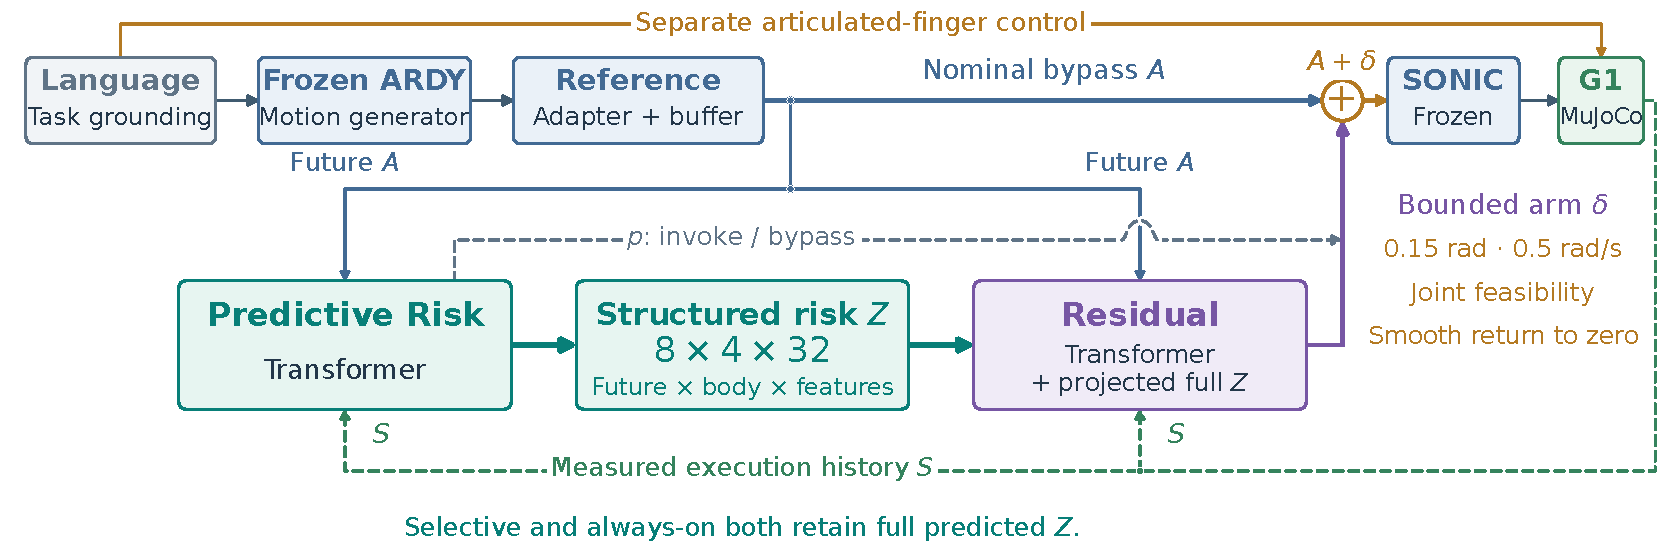
\includegraphics[width=\textwidth]{figures/architecture.pdf}
\caption{Structured predictive residual control, read from the nominal route at the upper left. Both learned models receive measured history $S$ and future nominal $A$. Risk transmits full $8\times4\times32$ tokens $Z$ to Residual (teal). The upper nominal route bypasses learned correction and feeds frozen SONIC at $A+\delta$. The scalar $p$ controls selective invocation on the correction branch: low risk skips Residual and requests zero, while an existing offset ramps down through the shared bounds and slew limit. Both invocation modes retain full predicted $Z$; fingers follow separate task commands.}
\label{fig:architecture}
\end{figure*}

\subsection{Measured History and Structured Prediction}
At time $t$, the inputs are robot history $S_t$, nominal future $A_t$, and available phase/finger context $C_t$:
\begin{equation}
 S_t\in\mathbb{R}^{16\times119},\quad
 A_t\in\mathbb{R}^{8\times62},\quad
 C_t\in\mathbb{R}^{8\times23}.
\end{equation}
Sixteen 50\,Hz history samples span 0.30\,s from first to last. Features include joint positions and velocities, root orientation, base angular velocity, relative palm/object geometry, contacts, tracking error, and phase. Future nominal tokens contain 29 positions, 29 velocities, and a root quaternion. The currently available phase and 14 finger commands are repeated across the future context; inference does not read future realized phases. Eight future slots spaced by 0.04\,s extend to 0.28\,s.

The Risk model predicts
\begin{equation}
 (Z_t,p_t,\widehat{Y}_t)=\Risk(S_t,A_t,C_t),\qquad
 Z_t\in\mathbb{R}^{8\times4\times32}.
 \label{eq:risk}
\end{equation}
The four groups are left arm/hand, right arm/hand, torso, and lower body. Temporal and body indices preserve this structure while the token features are learned. Auxiliary heads predict tracking error, required-contact loss, balance instability, and intervention/onset labels. The full $Z_t$ supplies Residual with future-time and body-specific predictive context. The scalar $p_t$ separately schedules invocation in selective mode.

Linear projections embed 16 history tokens and 32 body/time tokens into a pre-norm temporal Transformer~\cite{transformer}. The encoder has two layers, width 128, eight attention heads, a 512-dimensional feed-forward block, GELU, and final layer normalization. Attention pooling supplies the intervention head. Risk has 431,077 parameters.

\subsection{Conditioned Correction and Smooth Execution}
When invoked, a second Transformer with the same backbone dimensions receives projected Risk tokens added to the nominal/context embeddings:
\begin{equation}
 U_t=\Res(S_t,A_t,C_t,Z_t),\qquad U_t\in\mathbb{R}^{8\times14}.
\end{equation}
The Residual model has 438,030 parameters and predicts the 14 arm-joint offsets. Other body-joint offsets are zero, while SONIC continues to control the whole body. The learned module retains the nominal reference and adjusts the arm configuration locally~\cite{residual}. Auxiliary tracking, contact, and balance objectives shape $Z_t$, whose complete predicted token tensor conditions Residual.

The gate is evaluated before Residual inference. When invoked, the requested offset is $\Delta A_t^{\mathrm{req}}=0.15\tanh(U_t/0.15)$:
\begin{align}
 g_t&=\mathbb{1}[p_t\geq0.30],\\
 \Delta A_t^{\mathrm{cmd}}&=
 \begin{cases}
 \Delta A_t^{\mathrm{req}}, & g_t=1,\\
 0, & g_t=0.
 \end{cases}
\end{align}
Always-on mode sets $g_t=1$ while retaining Risk inference and the same $Z_t$ conditioning. At approximately 10\,Hz the controller predicts a horizon, executes the next step, and observes feedback again. The effective offset also passes through a shared magnitude/rate limiter:
\begin{equation}
 \delta_t=\delta_{t-1}+\operatorname{clip}
 (\bar{\delta}_t-\delta_{t-1},-0.5\Delta t,0.5\Delta t),
 \quad |\delta_t|\leq0.15,
 \label{eq:limiter}
\end{equation}
where angles are in radians and $\bar{\delta}_t$ is the magnitude-limited request. The production implementation checks horizon and nominal-relative velocities as well. Below the invocation threshold, the controller requests zero; an existing offset decays through the same rate limit. The last predicted slot is held over the remaining SONIC lookahead until replaced. This receding-horizon loop provides bounded local adaptation without retraining the generator or SONIC.

\section{Data and Supervised Learning}
\subsection{Causal Supervision}
We collect nominal executions and corrective teacher branches with their parent scene, measured state, reference inventory, and control settings. The Residual view has three supervision classes. \emph{Verified recovery} pairs a failed nominal continuation with a successful corrected continuation at the exact intervention state. \emph{Behavior cloning (BC)} uses later teacher states with their own measured histories. \emph{Stable identity} requests zero correction on stable nominal execution. Exact intervention-state pairs teach recovery; subsequent teacher states teach how to sustain the corrected execution.

Targets are absolute requested arm offsets before the shared limiter, matching the runtime interface. The Risk view uses nominal execution with valid future labels. Normalization is fitted to Risk TRAIN nominal data and reused for validation and Residual training. Residual is conditioned on its frozen matching Risk model's predictions, matching deployment.

\begin{table}[t]
\centering
\caption{Data and training}
\label{tab:training}
\begin{tabular}{lrr}
\toprule
 & Risk & Residual\\
\midrule
TRAIN parent executions & 3,163 & 1,917\\
TRAIN windows & 695,381 & 489,888\\
VAL windows & 1,946 & 1,832\\
Epochs run / retained epoch & 19 / 7 & 45 / 33\\
Optimizer updates & 4,864 & 23,040\\
Best validation objective & 0.188121 & 0.000344\\
Parameters & 431,077 & 438,030\\
\bottomrule
\end{tabular}
\end{table}

\subsection{Losses and Optimization}
Risk uses masked multi-task supervision,
\begin{equation}
 \mathcal{L}_{G}=\mathcal{L}_{\mathrm{int}}
 +2(\mathcal{L}_{\mathrm{track}}+\mathcal{L}_{\mathrm{contact}}
 +\mathcal{L}_{\mathrm{balance}})+0.25\mathcal{L}_{\mathrm{onset}}.
\end{equation}
Tracking uses MSE; contact, balance, intervention, and onset use valid-label BCE. Onset supervision distinguishes an upcoming event from a currently active violation. The Residual objective combines correction, BC, identity, and temporal smoothness:
\begin{equation}
 \mathcal{L}_{R}=\mathcal{L}_{\mathrm{corr}}+\mathcal{L}_{\mathrm{BC}}
 +2\mathcal{L}_{\mathrm{id}}+0.1\mathcal{L}_{\mathrm{smooth}}.
\end{equation}
Correction and BC emphasize the action actually executed by receding-horizon control: 0.8 first-step error plus 0.2 weighted-horizon error. Each loss has its own availability mask and denominator. Sampling first chooses supervision kind and parent origin, then a branch and window; BC/identity/recovery masses are 0.2/0.4/0.4. Verified recovery occupies only 1,055 of 489,888 windows (0.22\%): the exact intervention state is brief, whereas continuation produces many later samples. Assigning 40\% of draws to recovery gives these decision points substantial learning weight. BC supplies sustained corrective behavior, identity supplies stable continuation, and origin balancing limits domination by long branches.

Training uses Moore Threads S4000 accelerators and MUSA/PyTorch. AdamW~\cite{adamw} uses learning rates $10^{-4}$/$2\times10^{-4}$ and batch sizes 128/64 for Risk/Residual. Each epoch draws 32,768 samples; early stopping follows 12 epochs without validation improvement. Table~\ref{tab:training} reports actual training duration and retained checkpoints. Overlapping windows are training samples; parent executions identify source origins. Validation is fixed at eight nominal origins, of which seven supply admitted Residual parents. The appendix gives the supervision masks, sampling details, and recorded learning curves.

\section{Evaluation and Results}
\subsection{Evaluation Protocol}
\paragraph{Task success and recorded metrics}
A successful grasp requires opposing thumb/finger contact, block-bottom clearance of at least 0.05\,m, and at least 2\,s of continuous qualifying hold, followed by retention through the episode's final 5\,s hold. Sticky post-lift loss, prohibited contact, or a fall makes the trial unsuccessful. The 200\,Hz evaluator records contact and first-event evidence. Saved 50\,Hz states support continuous-history and rendering checks. Human correction count excludes automatic coordinator replans.

All experiments, including simulation data collection, model training, and evaluation, run on the course-provided Moore Threads S4000 cluster. The generator study uses the recorded 100-trial batch for each method. It measures grasp success, command-to-first-reference wall time, joint tracking RMSE, and user corrections under the common task implementation. The learned-controller confirmation is a separate ARDY-based experiment. Its baseline disables learned arm correction; Ours adds Risk-conditioned Residual control with the same SONIC, fingers, coordinator, scene initialization, and task criteria.

\paragraph{Independent paired confirmation}
The confirmation fixes 128 prospective origins. Each supplies an unscored nominal anchor and two scored arms, with order alternating by the original origin index. The reference policy is \emph{symmetric hybrid}: covered requests use a shared frozen reference inventory; uncovered requests generate from each branch's own measured state under the same rule. Reach, lower, and lift durations are 3.2, 3.2, and 4.8\,s. Model weights and runtime settings are frozen before the cohort.

Complete end-to-end pairs are the primary units. A scored operational failure counts as unsuccessful. A common anchor rejection leaves both scored arms unattempted and missing; there are no replacement scenes. The paired analysis uses recorded task events, synchronized execution clocks, and matching scene initialization. For $r$ rescues and $h$ harms among $n$ complete pairs, the estimated difference is $(r-h)/n$. The exact two-sided McNemar test~\cite{mcnemar} uses the prespecified family-wise allocation $\alpha=0.00625$. A paired-origin percentile interval~\cite{bootstrap} uses 100,000 resamples with RNG seed 261010. The interval is a nominal 95\% interval, separate from the multiplicity-controlled test.

\label{sec:results}
\subsection{ARDY versus Kimodo: 100 Trials per Method}
\begin{figure*}[t]
\centering
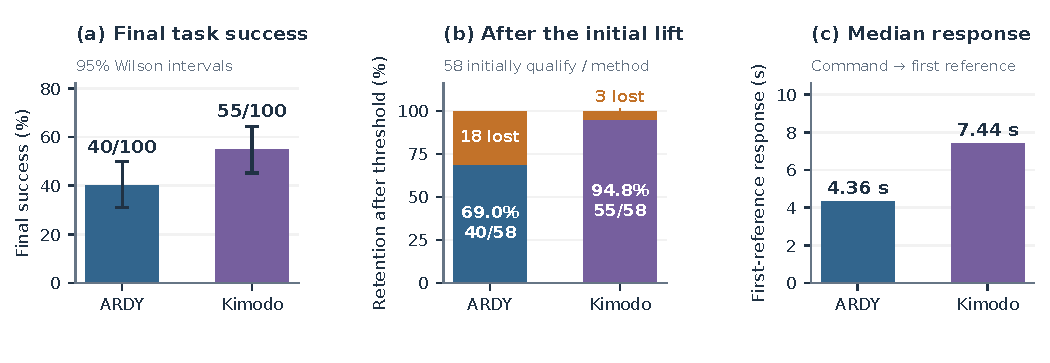
\includegraphics[width=\textwidth]{figures/generator-comparison.pdf}
\caption{Generator comparison on 100 shared scenes. Both methods initially meet the grasp threshold in 58 trials, but their subsequent retention differs. The middle panel conditions on each method's own 58 threshold-reaching trials; orange segments indicate later sticky losses. Final-success error bars are within-method 95\% Wilson intervals. Response is command-to-first-reference time.}
\label{fig:generators}
\end{figure*}

We evaluate both frozen generators on the same 100 scene requests (seeds 60000--60099), with common stage instructions, block positions, SONIC settings, finger gains, and automatic alignment replans. Each adapter retains its calibrated wrist convention. All scheduled attempts are included, with zero additional user corrections.

\begin{table}[t]
\centering
\caption{Generator comparison}
\label{tab:generators}
\begin{tabular}{lrr}
\toprule
 & ARDY+SONIC & Kimodo+SONIC\\
\midrule
Successful grasps & 40/100 & 55/100\\
Initial threshold & 58/100 & 58/100\\
Later sticky loss & 18/58 & 3/58\\
Wilson 95\% interval & 30.94--49.80\% & 45.24--64.39\%\\
Median initial response & 4.36\,s & 7.44\,s\\
Mean initial response & 4.78\,s & 7.77\,s\\
Mean joint RMSE & 0.0924\,rad & 0.0955\,rad\\
User corrections/trial & 0 & 0\\
\bottomrule
\end{tabular}
\end{table}
Response is command-to-first-usable-reference wall time, including setup, and is separate from learned-controller timings.

Kimodo achieves 55\% success versus ARDY's 40\%, an observed 15 percentage-point advantage (Table~\ref{tab:generators}). There are 23 shared successes, 28 shared failures, 32 Kimodo-only successes, and 17 ARDY-only successes. ARDY produces the first reference faster and attains slightly lower joint-tracking RMSE, while Kimodo converts more executions into retained grasps.

\paragraph{Initial lifting versus sustained manipulation}
\emph{Each generator reaches the clearance-and-contact threshold in 58/100 trials}. At the aggregate level, the 15-point final-success gap equals the 15-trial difference in later losses: $58-18=40$ for ARDY and $58-3=55$ for Kimodo. Conditional retention within each method's threshold-reaching trials is 69.0\% and 94.8\%, respectively. ARDY tracks joints slightly more accurately, yet loses more established grasps. Contact-compatible continuation therefore reveals manipulation quality that joint-tracking error alone misses. Of ARDY's 18 sticky losses, 16 receive the terminal reason \texttt{grasp\_lost\_after\_success} and two terminate with prohibited contact.

\paragraph{Motion locality and grasp geometry}
In the representative videos, ARDY couples right-hand motion with a more pronounced backward lean of the torso, away from the table, while Kimodo remains more upright and concentrates its adjustments in the arm. Such whole-body coupling changes wrist--object geometry during closing and holding. Shared finger gains and SONIC stabilization make contact-compatible reference motion a useful complement to joint-tracking accuracy.

\paragraph{Alignment versus acquisition}
\emph{Alignment miss} means that the measured block center never enters the hand's acquisition region during lowering and up to two feedback replans. Both methods use the same wrist-frame gate: $\pm4.5$\,cm laterally and $\pm1$\,cm vertically around the hand center. ARDY enters this region in 98 trials; two stop earlier with execution/contact errors. Kimodo enters in 72, while 28 exhaust both replans. Geometric readiness precedes finger closure and does not guarantee opposing contact: ARDY still has 17 acquisition failures, 18 timeouts, and later losses; Kimodo records four acquisition failures, nine timeouts, and three later losses. ARDY's zero alignment-miss count thus reflects an earlier-stage distinction rather than uniformly better grasping.

\begin{figure*}[t]
\centering
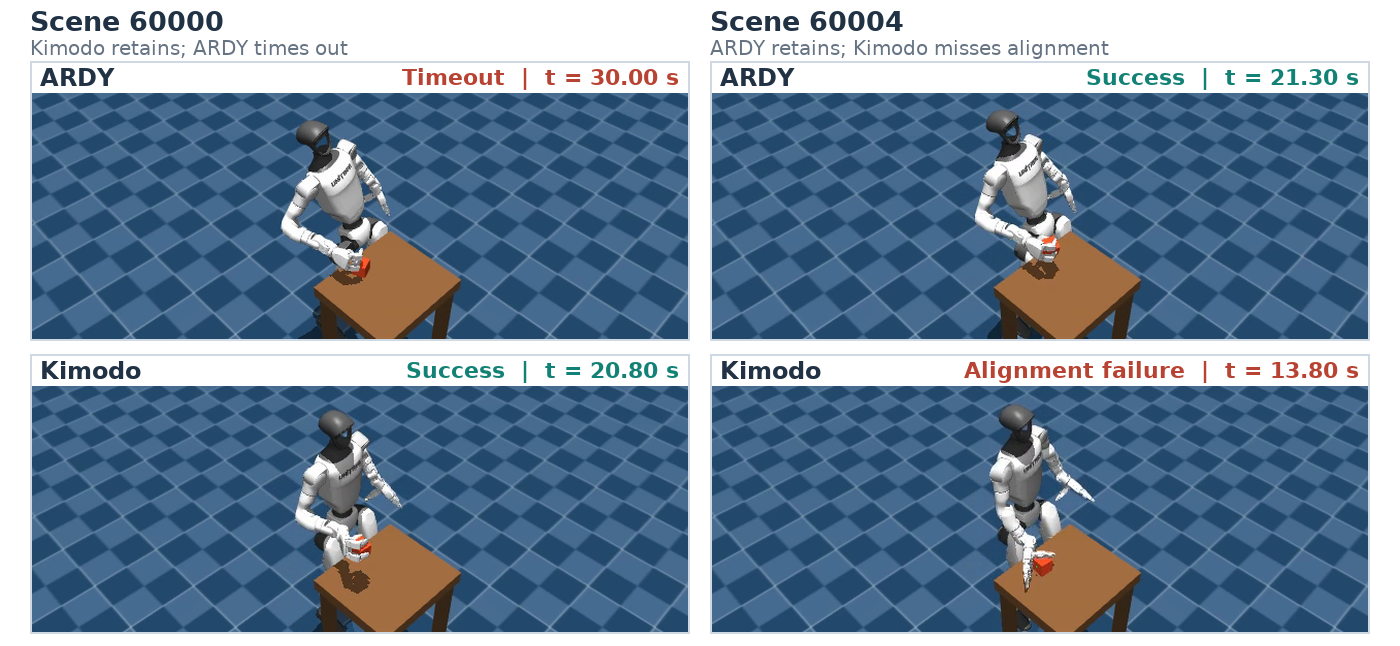
\includegraphics[width=\textwidth]{figures/baseline-qualitative.png}
\caption{Complementary outcomes in the 100-origin generator benchmark. In scene 60000, Kimodo succeeds while ARDY times out; in scene 60004, ARDY succeeds while Kimodo misses alignment. Frames show the final recorded physical state and simulation timestamp.}
\label{fig:baseline-qualitative}
\end{figure*}

Figure~\ref{fig:baseline-qualitative} illustrates this complementarity: generator choice changes the outcome on 49 scenes, and at least one method succeeds on 72. Aggregate ranking is therefore an incomplete guide to individual scenes. ARDY's faster response, measured-history conditioning, and feedback replanning motivate adding a local execution controller to improve acquisition and retention while preserving the nominal generator.


\subsection{Independent Evaluation of the Learned Extension}
\begin{figure*}[t]
\centering
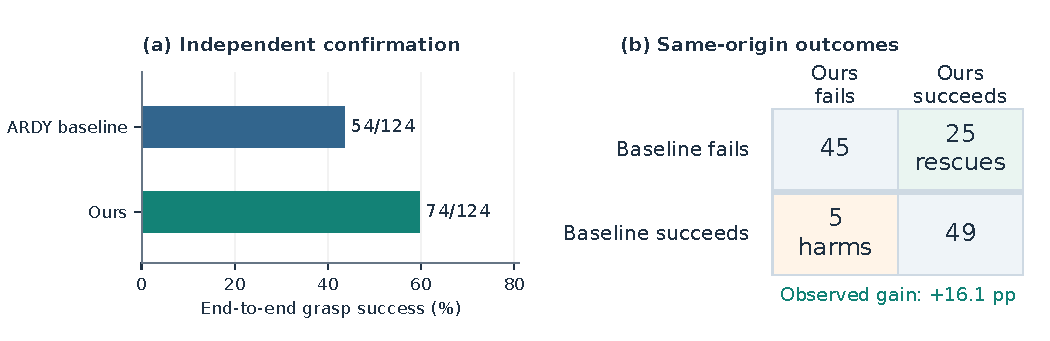
\includegraphics[width=\textwidth]{figures/confirmation.pdf}
\caption{Independent ARDY-based confirmation. Ours increases end-to-end success from 54 to 74 on 124 complete pairs. The paired outcomes reveal 25 rescues and five harms, with 49 shared successes and 45 shared failures. Four additional scheduled origins have common-anchor rejection and unattempted scored arms.}
\label{fig:confirmation}
\end{figure*}

Of 128 scheduled origins, 124 have complete end-to-end pairs and four have common nominal-reference rejection. The 248 scored attempts yield 54 baseline successes (43.55\%) and 74 successes for Ours (59.68\%). The gain is $+16.13$ percentage points, or 37.04\% relative to baseline. The paired table has 25 rescues, five harms, 49 shared successes, and 45 shared failures (Fig.~\ref{fig:confirmation}). Ours recovers 25 of the 70 baseline failures (35.7\%) and preserves 49 of the 54 baseline successes (90.7\%). The net gain of 20 successful origins combines failure recovery with preservation of already working behavior.

The exact result is $p=0.0003249142<0.00625$, satisfying the prospective decision rule. The nominal paired 95\% interval is $[+8.06,+24.19]$ percentage points. One operational failure of Ours counts as unsuccessful end-to-end; both methods fail at that origin. Across all 128 scheduled origins, assigning every possible outcome to the four unresolved pairs gives empirical effect bounds of $[+12.50,+18.75]$ percentage points. The all-origin effect remains positive across these missing-outcome assignments. The appendix distinguishes these identification bounds from the complete-pair confidence interval.

\subsection{Invocation Policies with Shared Risk Conditioning}
\begin{figure*}[t]
\centering
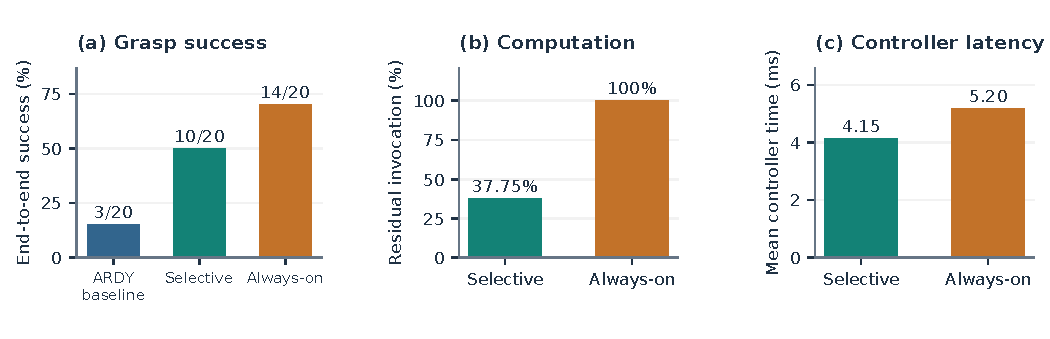
\includegraphics[width=\textwidth]{figures/gating.pdf}
\caption{Both learned configurations retain the same structured Risk-to-Residual pathway; the changed factor is Residual invocation. On 20 shared origins, always-on attains higher observed success, while selective invocation reduces Residual calls and controller latency. Learned weights are matched.}
\label{fig:gating}
\end{figure*}

The ablation compares ARDY baseline, selective correction at threshold 0.30, and always-on correction on a separate shared 20-origin cohort using a fixed checkpoint pair shared by the two learned arms and distinct from the confirmation checkpoints. Successes are 3/20 (15\%), 10/20 (50\%), and 14/20 (70\%), respectively. Relative to baseline, selective has seven rescues and no harms, and always-on has 11 rescues and no harms. Comparing the learned modes directly gives five always-on rescues and one always-on harm.

Both learned modes compute Risk and pass its complete predicted tokens to the same Residual model. Always-on therefore provides continuous Risk-conditioned correction. The scalar score controls whether Residual is called, while structured tokens condition what correction it requests. Higher observed always-on success favors continuous availability of that predictive feedback in this cohort; selective invocation trades some of this availability for fewer calls. Two origins produce native lower-replan reference-guard failures in both learned arms; all four operational failures count as unsuccessful in the 20-origin end-to-end endpoint. This ablation is interpreted descriptively.

\paragraph{Computation--success trade-off}
Selective execution invokes Residual on 1,575 of 4,172 Risk decisions (37.75\%), skipping 62.25\% of calls. Always-on invokes both models on all 4,075 decisions. Mean learned-controller time falls from 5.198 to 4.152\,ms: a 20.13\% reduction, or 1.046\,ms per decision. Median/P95 times are 3.525/5.216\,ms for selective and 5.127/6.062\,ms for always-on. Timings include controller preparation and learned inference on each arm's own evolving trajectory, separate from generation, SONIC, physics, and rendering.

Risk and preparation run in both modes, so skipping Residual saves part of the controller work. Both fit the 100\,ms decision interval; always-on has higher observed success, while selective invocation reduces computation.

\subsection{Failures and Qualitative Evidence}


\paragraph{Contact, clearance, and retention}
Grasping has a sequence of geometric bottlenecks. The hand must first enter the closure region, establish opposing contact, and then maintain a compatible wrist orientation while lifting. A small tracking error can coexist with a poor contact configuration; conversely, a local reference offset can improve object interaction while slightly changing joint tracking. The failure categories distinguish these stages and explain why success requires full-episode retention.

Figures~\ref{fig:retention-example} and~\ref{fig:qualitative}, together with the paired videos, make the correction effect concrete. At origin 76948, baseline reaches a 2.09\,s qualifying hold but later loses the block; Ours retains it with a 7.395\,s qualifying segment. At origin 77228, baseline succeeds with a 7.82\,s hold, while the corrected branch drops after a 4.315\,s segment. At shared-failure origin 76924, the corrected branch attains 0.071\,m clearance but only 1.305\,s of qualifying hold. These examples make sustained retention the decisive observable; peak block height alone misses both the recovery and the harmful correction.


% Task allocation table. Parent chooses final placement.
\begin{table*}[t]
\centering
\caption{Team contributions}
\label{tab:team-contributions}
\begingroup
\fontsize{9}{10.6}\selectfont
\setlength{\tabcolsep}{4pt}
\renewcommand{\arraystretch}{1.0}
\begin{tabular}{@{}p{0.27\textwidth}p{0.71\textwidth}@{}}
\toprule
Task & Team members\\
\midrule
Archon session & All group members\\
Simulation and SONIC & Sun Yuhan, Tie Yutong, Gu Wentao, Wang Qifa\\
ARDY integration & Wang Yuxiang, Xia Fangxin, Yin Siyuan, Gu Wentao\\
Kimodo integration & Tie Yutong, Zang Ziyi, Zhu Jianyu, He Yutong\\
Execution data and labels & Lu Yinuo, Sun Yuhan, Wang Yuxiang, Gu Wentao\\
Risk/Residual models & Gu Wentao, Shi Yixin, Tie Yutong, Xia Fangxin\\
Training and optimization & Wang Qifa, Gu Wentao, Yin Siyuan, Zang Ziyi\\
Evaluation and ablations & Zhu Jianyu, He Yutong, Gu Wentao, Lu Yinuo\\
Video rendering and slides & Shi Yixin, Sun Yuhan, Yin Siyuan, Gu Wentao\\
Report and figures & Wang Qifa, Xia Fangxin, Gu Wentao, Zang Ziyi, Zhu Jianyu\\
\bottomrule
\end{tabular}
\endgroup
\end{table*}


\paragraph{Correction authority and remaining failures}
Native joint-range rejection exposes a second interface bottleneck: a generated whole-body motion can be unacceptable before SONIC installs it. Arm-only correction has authority over contact geometry after reference acceptance, while the generator adapter must handle lower-body feasibility. The end-to-end endpoint includes both kinds of failure.

The five harms show that bounded correction can worsen an otherwise successful execution. Preserving stable contact is therefore a distinct objective alongside recovering failures.

% Start the discussion below the final-page contribution table.
\newpage
\section{Discussion and Limitations}
The experiments identify two complementary design questions: whether nominal motion remains compatible with object contact, and how corrective control uses execution feedback. Equal initial threshold counts conceal a large retention gap between generators. Our extension addresses execution through a structured intermediate representation: future-time and body indices organize predicted features before Residual maps them to local corrections. The scalar gate compresses invocation into one decision, while the full tensor retains context for correction. Always-on keeps this information path continuously available. Its observed advantage makes invocation a task-utility decision, alongside the design of the predictive representation.

\paragraph{Scope and limitations}
The experiments cover staged right-hand lifting of one block family with simulator-grounded object state. New shapes, payloads, bimanual tasks, and estimated visual state remain open. Generation pauses simulated time; real-robot deployment requires asynchronous planning and measured sensing/control delays beyond the learned-component timing. Eight nominal validation origins provide limited diversity despite the larger training set.

The confirmation evaluates the complete Risk-conditioned controller, while the invocation study isolates scheduling with full $Z_t$ retained. Matched binary-, scalar-, body-vector-, and full-token studies should quantify the contribution of risk structure. Corrections affect only the arms; the five harms show that magnitude/rate bounds alone do not ensure useful contact changes. These interfaces and contact-preservation behavior need evaluation across tasks.


The public \href{https://github.com/Peneplain/dl}{implementation repository} provides configurations, setup instructions, and evaluation code.

The \href{https://github.com/Peneplain/dl/tree/main/report}{report source} provides the editable manuscript and figures; the \href{https://github.com/Peneplain/dl/tree/main/docs/results}{numerical supplement} records learning curves, summaries, and source hashes. Annotated success/failure videos for both generators and the learned extension are available at \url{https://github.com/Peneplain/dl/tree/main/videos}. We acknowledge ARDY, Kimodo, GEAR-SONIC/GR00T-WholeBodyControl, Unitree G1 assets, Llama~\cite{llama3}/LLM2Vec, and MuJoCo. LLM assistance supported implementation and drafting; external materials retain their original licenses.

% Keep the conclusion together in the final right-hand column.
\newpage
\section{Conclusion and Future Outlook}
Two motion generators share one SONIC execution pipeline, yet differ in response time, alignment, and retention. Our learned extension transmits structured predictions of future execution from Risk to Residual, linking anticipation to bounded arm correction. This Risk-conditioned controller improves the ARDY-based system from 43.55\% to 59.68\% success in an independent paired evaluation. Both continuous and selective invocation retain the predictive interface. Table~\ref{tab:team-contributions} gives the team task allocation.

\begin{figure}[h]
\centering
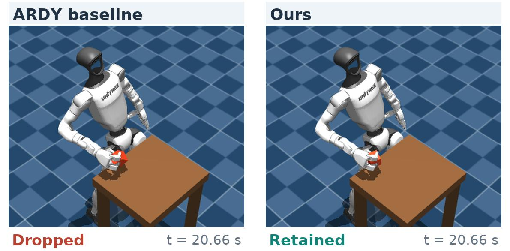
\includegraphics[width=\columnwidth]{figures/retention-example.pdf}
\caption{Contact retention at origin 76948. Baseline loses the block after a 2.09\,s qualifying segment; Ours retains it through final assessment. Both images show the original terminal state at 20.66\,s.}
\label{fig:retention-example}
\end{figure}

Future work will evaluate this controller on a physical G1 under supervision, using visual state estimation, calibrated timing, and measured contact feedback. Object placement, bimanual handling, and transport will test whether the learned interface transfers beyond tabletop lifting. Integrating a vision-language-action (VLA) policy, such as OpenVLA~\cite{openvla}, upstream will extend visual and instruction conditioning while retaining the structured Risk-to-Residual interface. Dynamics randomization~\cite{dynamics_randomization} offers a route to stress-test friction, payload, and actuator mismatch before hardware trials. More diverse objects, task conditions, and validation origins will support this progression.

\label{body:end}
\clearpage
\bibliographystyle{IEEEtran}
\bibliography{references}
\clearpage
\appendices
% Allow paired appendix figures to share the page with supporting text.
\renewcommand{\dbltopfraction}{0.86}
\renewcommand{\textfraction}{0.10}
\setcounter{dbltopnumber}{2}

\section{Training Details}
Residual TRAIN contains 1,055 verified-correction, 311,945 causal teacher-BC, and 176,888 stable-identity windows, totaling 489,888 from 1,917 distinct parents; parent classes may overlap. Risk has 695,381 windows from 3,163 nominal TRAIN parents. Validation has eight nominal parents and seven admitted Residual parents.

Risk draws 5\% recovery-associated and 95\% background samples with parent balancing. Residual draws BC/identity/recovery at masses 0.2/0.4/0.4, then chooses an origin, branch, and window. Each epoch draws 32,768 samples with replacement; these draws add optimizer updates, not independent origins.

Risk/Residual AdamW weight decays are 0.02/0.01 and dropouts 0.20/0.10. Gradient clipping is 1.0, the maximum budget is 60 epochs, and patience is 12. Retained checkpoints are epoch 7 of 19 and epoch 33 of 45. Matching Risk remains frozen throughout Residual training.

Correction and BC use $0.8\mathcal{L}_{\mathrm{first}}+0.2\mathcal{L}_{\mathrm{horizon}}$ with horizon weights $[4,3,2,1,1,1,1,1]$. Identity penalizes requested offsets; smoothness penalizes adjacent horizon differences, each with its availability mask. Targets are absolute pre-limiter requests, not increments to effective offsets.

Tracking uses masked MSE. Required-contact loss means opposing right-hand contact loss during lift/hold. Contact, balance, intervention, and onset use valid-label BCE; onset excludes current violations and verified-recovery windows. Teacher-BC states supply no nominal Risk labels.

\begin{figure*}[p]
\centering
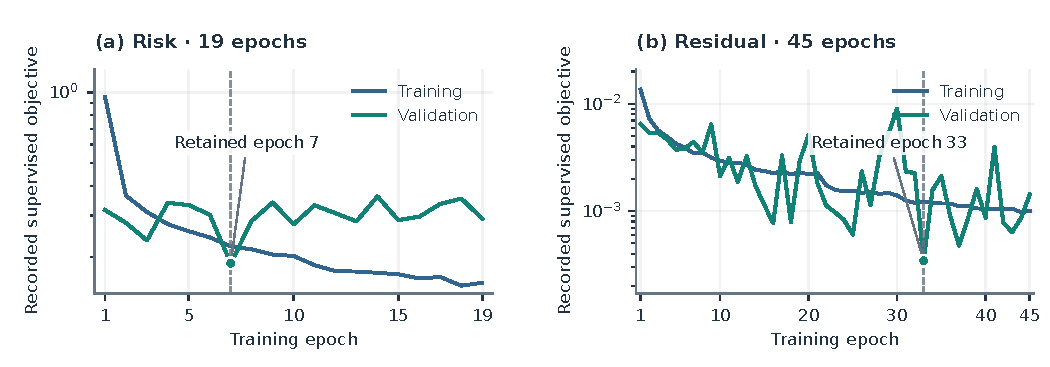
\includegraphics[width=0.94\textwidth]{figures/learning-curves.pdf}
\caption{Recorded optimization histories. Retained checkpoints follow validation objectives; task improvement is measured separately in simulated execution.}
\vspace{3pt}
\begin{minipage}[t]{0.48\textwidth}
\centering
\vspace{0pt}
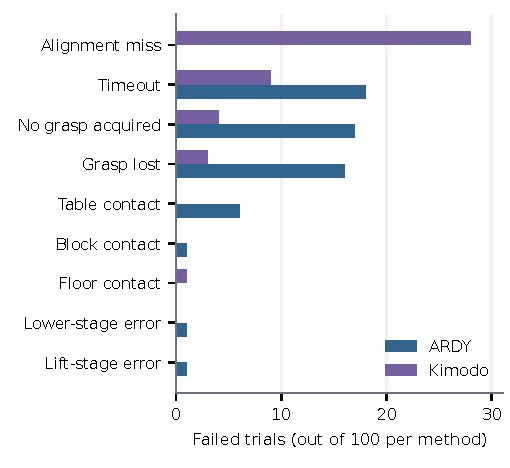
\includegraphics[width=0.83\linewidth]{figures/failure-profile-column.pdf}
\caption{Terminal failure categories for the shared 100-origin generator benchmark, including every unsuccessful trial.}
\end{minipage}\hfill
\begin{minipage}[t]{0.48\textwidth}
\vspace{6pt}
\centering
{\makeatletter\def\@captype{table}\caption{Terminal failure categories}\makeatother}
\begin{tabular}{lrr}
\toprule
Terminal reason & ARDY & Kimodo\\
\midrule
Alignment missed & 0 & 28\\
Grasp not acquired & 17 & 4\\
Timeout & 18 & 9\\
Loss after success threshold & 16 & 3\\
Prohibited robot--table contact & 6 & 0\\
Prohibited robot--block contact & 1 & 0\\
Block--floor contact & 0 & 1\\
Lower/lift execution error & 2 & 0\\
\midrule
Total unsuccessful & 60 & 45\\
\bottomrule
\end{tabular}

\vspace{4pt}
\small Each unsuccessful trial has one terminal reason. The chart separates lower- and lift-stage errors; the table combines those two categories.
\end{minipage}
\par\vspace{9pt}
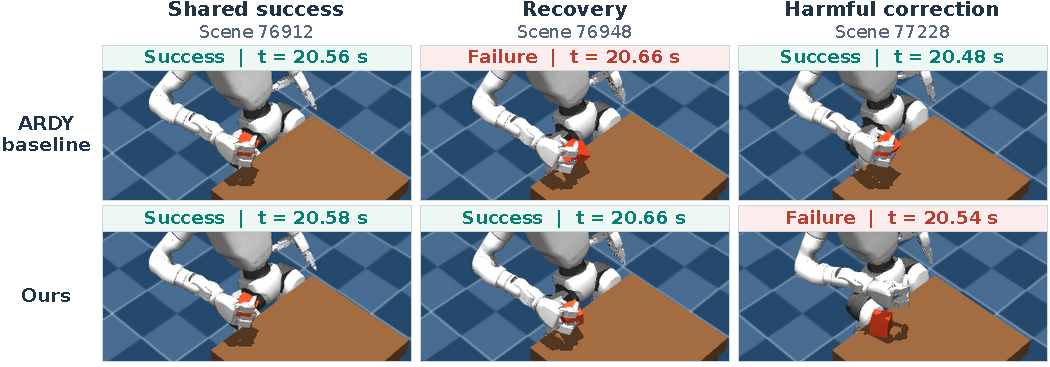
\includegraphics[width=\textwidth]{figures/qualitative-compact.pdf}
\caption{Paired execution examples: shared success, recovery, and harmful correction. Contact-focused crops show recorded final states; labels give the whole-episode outcome and simulation time. Videos show the preceding lift and retention sequence.}
\label{fig:qualitative}
\end{figure*}

\section{Paired Evaluation Details}
The confirmation schedules $76912+4i$, $i=0,\ldots,127$. Origins 76992, 77144, 77304, and 77416 reject the common nominal anchor; both scored arms remain unattempted. An operational failure of Ours at 77256 counts as unsuccessful; baseline also fails. The 124 end-to-end pairs give 49 shared successes, 45 shared failures, 25 rescues, and five harms. The descriptive completed-physical subset has 123 pairs and successes 54/123 versus 74/123.

The success-rate difference is $(25-5)/124\approx0.16129$, or 16.129 percentage points. The exact paired test uses prospective $\alpha=0.00625$ within a family of at most eight comparisons. The nominal 95\% percentile interval uses 100,000 paired-origin resamples and RNG 261010. Four unresolved pairs give empirical all-origin bounds of $[12.50,18.75]$ percentage points, obtained from $100(20-4)/128$ and $100(20+4)/128$; these missing-outcome bounds are distinct from confidence intervals.

Covered requests share cached references. Uncovered phases/durations generate from each branch's measured state under the same frozen rule. Order alternates by original origin index. This symmetric hybrid protocol permits feedback-dependent generation, with no replacement origins, repeated physical failures, or outcome-dependent extensions.

The separate invocation study schedules 20 origins and 60 scored arms. At 78196 and 78216, both learned arms fail native lower-replan joint-range checks; all four remain unsuccessful. Thus end-to-end successes are 3/20, 10/20, and 14/20; the descriptive 18-origin completed-physical subset gives 3/18, 10/18, and 14/18.

Selective makes 4,172 Risk calls and 1,575 Residual calls; always-on makes 4,075 of each. Mean Risk inference is 2.290/2.265\,ms; active Residual inference is 1.727/1.713\,ms. Controller means include preparation. Decisions follow each arm's own trajectory; task-level units remain origins.

\section{Generator Benchmark Details}
Both batches use the same requests and seeds 60000--60099; all paired scene hashes and SONIC manifests match. Block XY is sampled from $[0.36,0.46]\times[-0.30,-0.16]$\,m. Shared settings are direct standing start, 0.2\,m table standoff, open-hand approach, up to two automatic alignment replans, each capped at 1.6\,s, 0.3\,s acquisition transition, 4.8\,s lift, and 5\,s final hold. The acquisition gate tests measured block position in the wrist frame before closing; opposing contact is checked separately after closing. Finger gains are $K_P=6$, $K_D=0.4$. Kimodo uses calibrated wrist offset $(0.125,0.035,0.080)$\,m; ARDY uses its measured hand-center default. Response includes grounding, generation, and transition setup. Native 25/30\,Hz rates describe motion sampling rather than response throughput.

\section{Qualitative Evidence and Artifacts}
Figure~\ref{fig:qualitative} shows shared success at 76912, recovery at 76948, and harmful correction at 77228. Labels summarize whole-episode outcomes, including sticky loss; crops show final geometry. The video supplement at \url{https://github.com/Peneplain/dl/tree/main/videos} pairs instructions with execution stages, simulation time, and behavior for both generators and the extension. Its manifest records scenes, views, outcomes, sizes, and hashes. Saved 50\,Hz states support rendering; contacts are evaluated at 200\,Hz.

The \href{https://github.com/Peneplain/dl/tree/main/docs/results}{numerical supplement} contains complete benchmark outcomes, confirmation, learning curves, invocation/timing records, and source hashes. The \href{https://github.com/Peneplain/dl/tree/main/report}{report source} provides the complete editable manuscript and its figure assets.

\end{document}
